\documentclass[14pt, a4paper]{report}
\usepackage{mathtext}
\usepackage[T2A]{fontenc}
\usepackage[utf8]{inputenc}
\usepackage[russian]{babel}
\usepackage{multirow}
\usepackage{slashbox}
\usepackage{makecell}
\usepackage{graphicx}
\usepackage{physics}
\usepackage{amstext}
\usepackage{caption}
\usepackage{subcaption}

\renewcommand{\thesection}{\arabic{section}.}
\renewcommand{\thesubsection}{\arabic{section}.\arabic{subsection}.}

\title{\textbf{Отчет о выполнении лабораторной работы 3.5.1 "Изучение плазмы газового разряда в неоне"}}
\author{Алпатова Александра, Калашников Михаил, Б03-205}
\date{}

\begin{document}
\maketitle

\textbf{Цель работы:}
Изученние ВАХ тлеющего разряда; свойств плазмы методом зондовых характеристик.
\newline

\textbf{В работе используются:}
\begin{itemize}
\item стеклянная газоразрядная трубка, наполненная неоном;
\item высоковольтный источник питания;
\item источник питания постоянного тока;
\item делитель напряжения;
\item резистор;
\item потенциометр;
\item амперметры;
\item вольтметры;
\item переключатели. 
\end{itemize}

\section*{Теоретическая справка}

\textit{Двойным зондом} назывется система, состоящая их двух одинаковых зондов, расположенных на небольшом расстоянии друг от друга. Между зондами создаётся разность потенциалов $U$, которая по велиине много меньше плавающего потенциала: $\left|U\right|\ll\left|U_f\right|$. При этом оба зонда имеют относительно плазмы близкий к плавающему отрицательный потенциал, т.е. находятся на \textit{ионной} ветви вольт-амперной характеристики.

При отсутствии разности потенциалов ток между зондами равен нулю. Рассчитаем величину тока, проходящего через двойной зонд вблизи точки $I=0$. При небольших разностях потенциалов ионные токи на оба зонда равны ионному току насыщения и компенсируют друг друга. Величина результирующего тока целиком связана с различием в электронных токах. Пусть потенциал на первом зонде равен\[U_1=U_f+\Delta U_1,\]а на втором\[U_2=U_f+\Delta U_2.\]Предполагается, что $\Delta U_1,\Delta U_2\ll U_f$. Напряжение $U$ между зондами равно\[U=U_2-U_1=\Delta U_2-\Delta U_1.\]

Найдём ток, приходящий на первый электрод:\[I_1=I_{i\text{н}}-I_{e0}\exp{\left(\frac{eU_1}{k_{\text{Б}T_e}}\right)}=I_{i\text{н}}-\left[I_{e0}\exp{\left(\frac{eU_f}{k_{\text{Б}T_e}}\right)}\right]\exp{\left(\frac{e\Delta U_1}{k_{\text{Б}T_e}}\right)}.\]Заметим, что при $\Delta U_1=0$ (при $U_1=U_f$) электронный и ионный ток компенсируют друг друга. Это означает, что заключённый в квадратные скобки множитель равен $I_{i\text{н}}$. Имеем поэтому\[I_1=I_{i\text{н}}\left[1-\exp{\left(\frac{e\Delta U_1}{k_{\text{Б}T_e}}\right)}\right].\]Аналогично для второго электрода\[I_2=I_{i\text{н}}\left[1-\exp{\left(\frac{e\Delta U_2}{k_{\text{Б}T_e}}\right)}\right].\]

Заметим, что зонды 1 и 2 соединены \textit{последовательно} -- через плазму -- поэтому $I_1=-I_2=I$. Выразим $\Delta U_1$ и $\Delta U_2$ из уравнений выше:\[\Delta U_1=\frac{k_{\text{Б}}T_e}{e}\ln{\left(1-\frac{I}{I_{i\text{н}}}\right)},\ \Delta U_2=\frac{k_{\text{Б}}T_e}{e}\ln{\left(1+\frac{I}{I_{i\text{н}}}\right)}.\]Наконец, вычитая второе равенство из первого, найдём\[U=\Delta U_1-\Delta U_2=\frac{k_{\text{Б}}T_e}{e}\ln{\left(\frac{I_{i\text{н}}-I}{I_{i\text{н}}+I}\right)},\]и, разрешая это равенство относительно $I$, получим\[I=I_{i\text{н}}\th{\frac{eU}{2k_{\text{Б}}T_e}}.\]Эту формулу можно использовать для определния температуры электронов по форме вольт-амперной характеристики двойного зонда.

Наблюдаемая на опыте зависимость тока от напряжения изображена на рисунке 1. Заметим, что эта кривая отличается от теоретической существованием наклона у асимптот в области больших $\left|U\right|$, что связано с ускорением частиц плазмы приложенным полем, которое не учтено при выводе теоретической зависимости.

Графики типа 1 проще всего обрабатывать следующим образом. Сначала находится ток насыщения $I_{i\text{н}}$ из пересечения асимптот с осью $U=0$. Затем находится наклон графика в начале координат, из которого можно определить температуру электронов $T_e$. Дифференциируя формулу для $I$ по $U$ в точке $U=0$ и принимая во внимание, что при малых аргументах $\th{x}\approx x$, найдём\[k_{\text{Б}}T_e=\frac{1}{2}\frac{eI_{i\text{н}}}{\frac{\text{d}I}{\text{d}U}\vert{}_{U=0}},\]где $\frac{\text{d}I}{\text{d}U}\vert{}_{U=0}$ -- наклон характеристики зонда вблизи начала координат. По известным $T_e$ и $I_{i\text{н}}$ можно найти концентрацию заряженных частиц $n_i=n_e$.

Таким образом, двойные зонды удобно применять для измерения электронной температуры и концентрации частиц в плазме.

\begin{figure}[h]
	\centering
	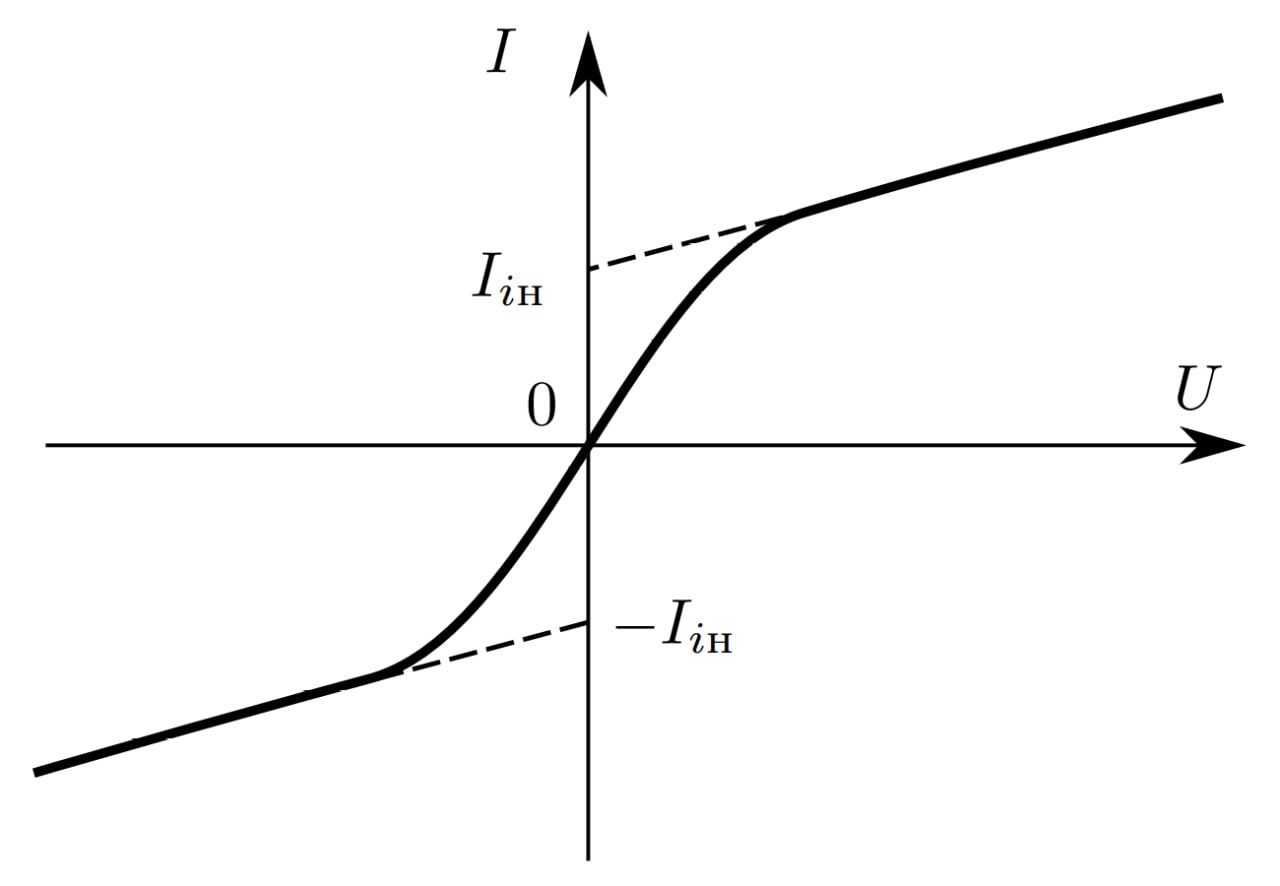
\includegraphics[scale=0.30]{images/351_6.jpg}
	\caption{Вольт-амперная характеристика двойного зонда} \label{Tok}
\end{figure}

\section*{Экспериментальная установка}

Схема установки для исследования плазмы газового разряда в неоне представлена на рисунке 2. Стеклянная газоразрядная трубка имеет холодный (ненагреваемый) полый катод, три анода и \textit{геттерный узел} -- стеклянный балон, на внутреннюю поверхность которого напылена газопоглощающая плёнка (\textit{геттер}). Трубка наполнена изотопом неона ${}^{22}\text{Ne}$ при давлении 2 мм рт. ст. Катод и один из анодов (I или II) с помощью переключателя $\text{П}_1$ подключаются через балластный резистор $R_{\text{б}}$ ($\sim450~\text{к}\Omega$) к регулируемому высоковольтному источнику питания (ВИП) с выходным напряжением до 5 кВ.


При подключении к ВИП анода-I между ним и катодом возникает газовый разряд. Ток разряда измеряется миллиамперметром $A_1$, а падение напряжение на разрядной трубке -- цифровым вольтметром $V_1$ (мультиметром GDM), подключённым к трубке через высоомный ($25~\text{М}\Omega$) делитель напряжения с коэффициентом $\frac{R_1+R_2}{R_2}=10$.

При подключении к ВИП анода-II разряд возникает в пространстве между катодом и анодом-II, где находится двойной зонд, используемый для диагностики плазмы положительного столба.

Зонды изготовлены из молибденовой проволоки диаметром $d=0,2~\text{мм}$ и имеют длину $l=5,2~\text{мм}$. Они подключены к источнику питания GPS через потенциометр $R$. Переключатель $\text{П}_2$ позволяет изменять полярность напряжения на зондах. Величина напряжения на зондах изменяется с помощью дискретного переключателя "$V$" выходного напряжения источника питания и потециометра $R$, а измеряется цифровым вольтметром $V_2$ (GMD). Для измерения зондового тока используется мультиметр $A_2$ (GDM). Анод-III в нашей работе не используется.

\begin{figure}[h]
\centering
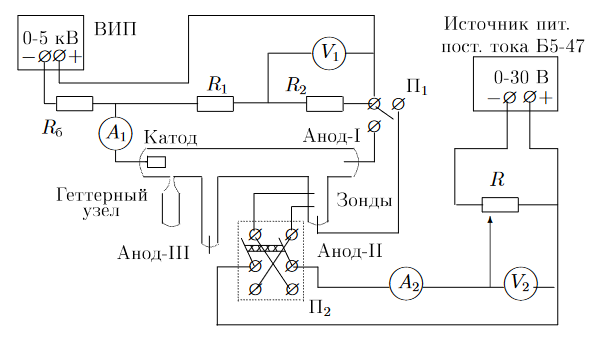
\includegraphics[scale=0.6]{images/351_5.png}
\caption{Схема установки для исследования газового разряда}
\end{figure}


\section{Проведение эксперимента}

\begin{enumerate}

\setcounter{enumi}{0}

\item Определим напряжение зажигания разряда по нескольким измерениям: $U_{заж}=206\pm8\ В$.

\item Проведем измерение ВАХ разряда. Полученные точки приведены на рис. 1.

\item[3-4.] Подготовим оборудование к измерению зондовых характеристик.

\setcounter{enumi}{4}

\item Проеведем измерения ВАХ двойного зонда в диапазоне от $-25\ В$ до $25\ В$ при токе разряда $I_р=5\ мА$.

\item Повторим предыдущие пункты для токов разряда $3\ мА$ и $1.5\ мА$.

\item Выключим все использовнное оборудование и зафиксируем параметры зондов: $d=0.2\ мм$, $l=5.2\ мм$.

\end{enumerate}

\section{Обработка данных}

\begin{enumerate}

\setcounter{enumi}{7}

\item Построим ВАХ разряда (рис. 2). Проведем прямую через точки, лежащие в правой нижней области и найдем маскмальное дифференциальное сопротивление разряда $R_{диф}=\dv{U}{I}=-3.1\pm0.2\ Ом$. Полученная зависимость вероятнее всего является частью участка Г-Д ВАХ разряда, представленной в лабнике.

\item Теперь построим зондовые характеристики для разных токов (рис. 3). Проведем касательную в нуле и асимптоты в бесконечностях чтобы определить производную $\left.\dv{I}{U}\right\vert_{U=0}$ и ток насыщения $I_{iн}$. После этого найдем температуру электронов в Кельвинах по формуле:
\[kT_e=\frac{1}{2}\frac{eI_{iн}}{\left.\dv{I}{U}\right\vert_{U=0}}\]

\item Результаты вычислений с погрешностями, полученные в предыдущем пункте и во всех последующих будут представлены в сводной таблице в коцне работы.

\item Вычислим концентрацию электронов с помощью формулы Бома, полагая, что $n_e=n_i$:
\[n_{e}=\frac{5}{2}\frac{I_{iн}}{e\pi ld}\sqrt{\frac{m_i}{2kT_e}}\]

\item Рассчитаем плазменную частоту колебаний электронов по формуле:

\[\omega_p=\sqrt{\frac{4\pi n_ee^2}{m_e}}=5.6\cdot10^4\sqrt{n_e}\ \frac{рад}{с}\]

Рассчитаем электронную поляризационную длину $r_{D_e}$ по формуле:

\[r_{D_e}=\sqrt{\frac{kT_e}{4\pi n_ee^2}}\]

Также найдем дебаевский радиус экранирования $r_D$, принимая температуру ионов равной комнатной ($T_i\approx300\ К$):

\[r_D=\sqrt{\frac{kT_i}{4\pi n_ee^2}}\]

\item Оценим среднее число ионов в дебаевской сфере:

\[N_d=\frac{4}{3}\pi r_D^3n_i\]

\item Оценим степень ионизации плазмы ($P\approx2\ торр$):

\[\alpha=\frac{n_i}{n}=\frac{n_ekT_i}{P}\]

\item Построим графики зависимостей электронной температурыи и концентрации электронов от тока разряда: $T_e(I_р)$, $n_e(I_р)$ (рис. 4 и рис. 5).

\item Ниже приведена сводная таблица полученных значений.

\end{enumerate}

\section{Вывод}

Дебаевский радиус электронов $r_{D_e}$ много меньше поперечного размера трубки, в котором содержится плазма. Поэтому последнюю можно считать квазинейтральной. Идеальной плазму можно считать с малой точностью, так как число Дебая $N_D$ не много больше 1.

\section{Приложения}

\begin{table}[h]
\centering
\makebox[\textwidth][c] {
\begin{tabular}{| c | c | c | c |}
\hline
$I_р,\ мА$ & $kT_e,\ эВ$ & $n_e,\ см^{-3}$ & $\omega_p,\ рад\cdot с^{-1}$ \\
\hline
5	 & $1.056\pm0.013$	 & $(1.288\pm0.018)\cdot10^{12}$	 & $(6.36\pm0.04)\cdot10^{10}$	 \\
3	 & $1.969\pm0.004$	 & $(5.126\pm0.014)\cdot10^{11}$	 & $(4.010\pm0.005)\cdot10^{10}$	 \\
1.5	 & $2.576\pm0.004$	 & $(2.161\pm0.004)\cdot10^{11}$	 & $(2.603\pm0.003)\cdot10^{10}$	 \\
\hline
\hline
$r_{D_e},\ см$ & $r_D,\ см$ & $N_D$ & $\alpha$ \\
\hline
$(6.74\pm0.06)\cdot10^{-4}$	 & $(1.054\pm0.007)\cdot10^{-4}$	 & $6.31\pm0.16$	 & $(2.03\pm0.03)\cdot10^{-5}$	 \\
$(1.457\pm0.003)\cdot10^{-3}$	 & $(1.670\pm0.002)\cdot10^{-4}$	 & $10.00\pm0.05$	 & $(8.06\pm0.02)\cdot10^{-6}$	 \\
$(2.567\pm0.003)\cdot10^{-3}$	 & $(2.572\pm0.003)\cdot10^{-4}$	 & $15.41\pm0.05$	 & $(3.400\pm0.007)\cdot10^{-6}$	 \\
\hline

\end{tabular}
}
\caption{Сводная таблица расчетов}
\end{table}

\begin{figure}[h]
\centering
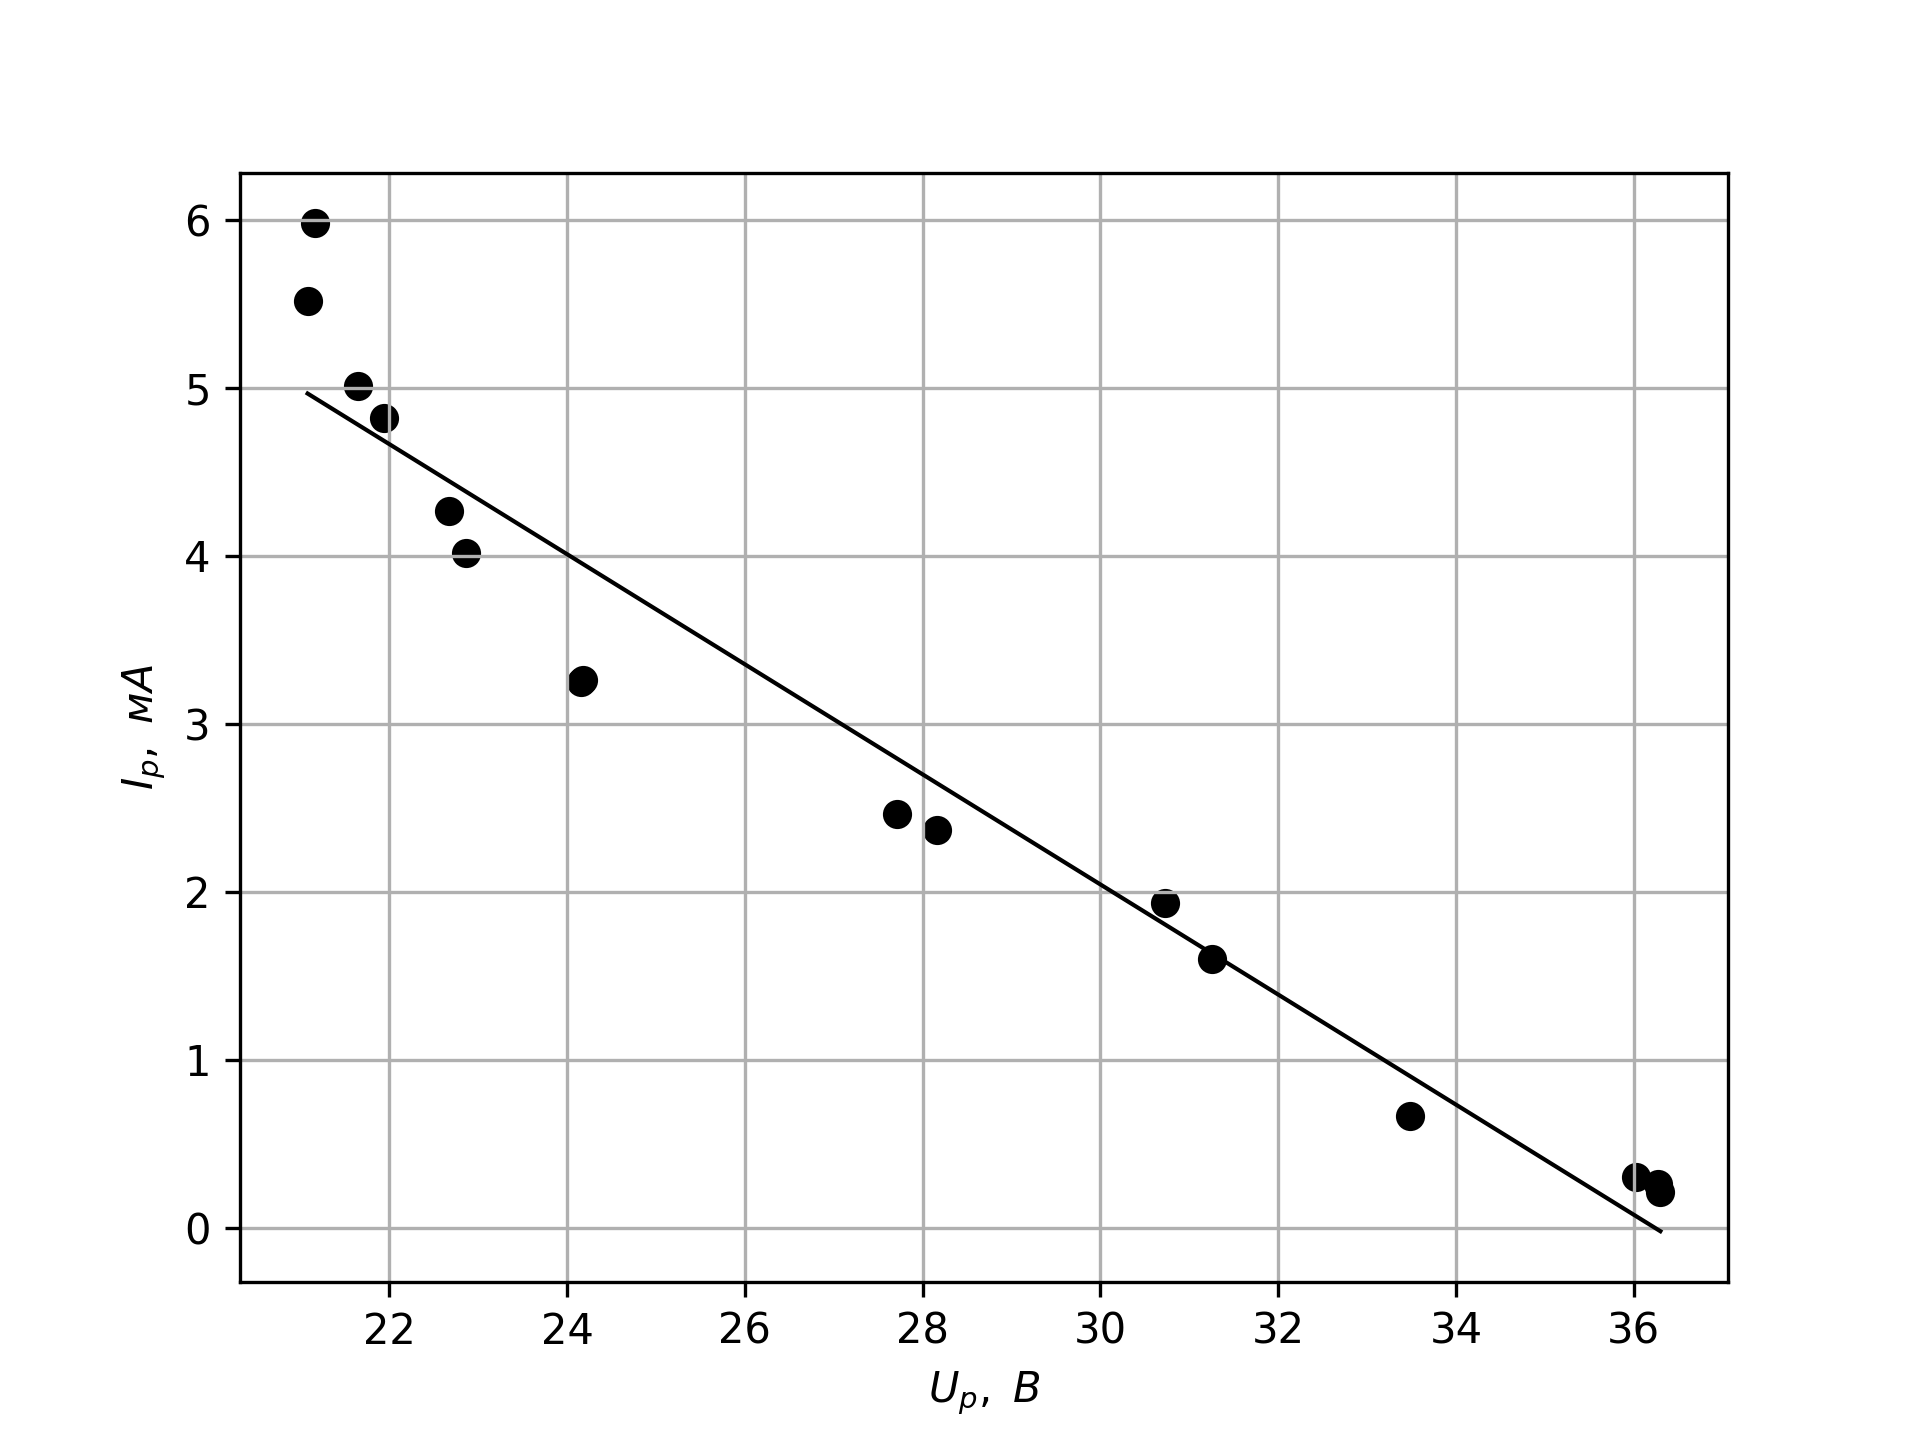
\includegraphics[scale=0.6]{images/351_1.png}
\caption{Вольт-амперная характеристика разряда $I_р(U_р)$}
\end{figure}

\begin{figure}[h]
\centering
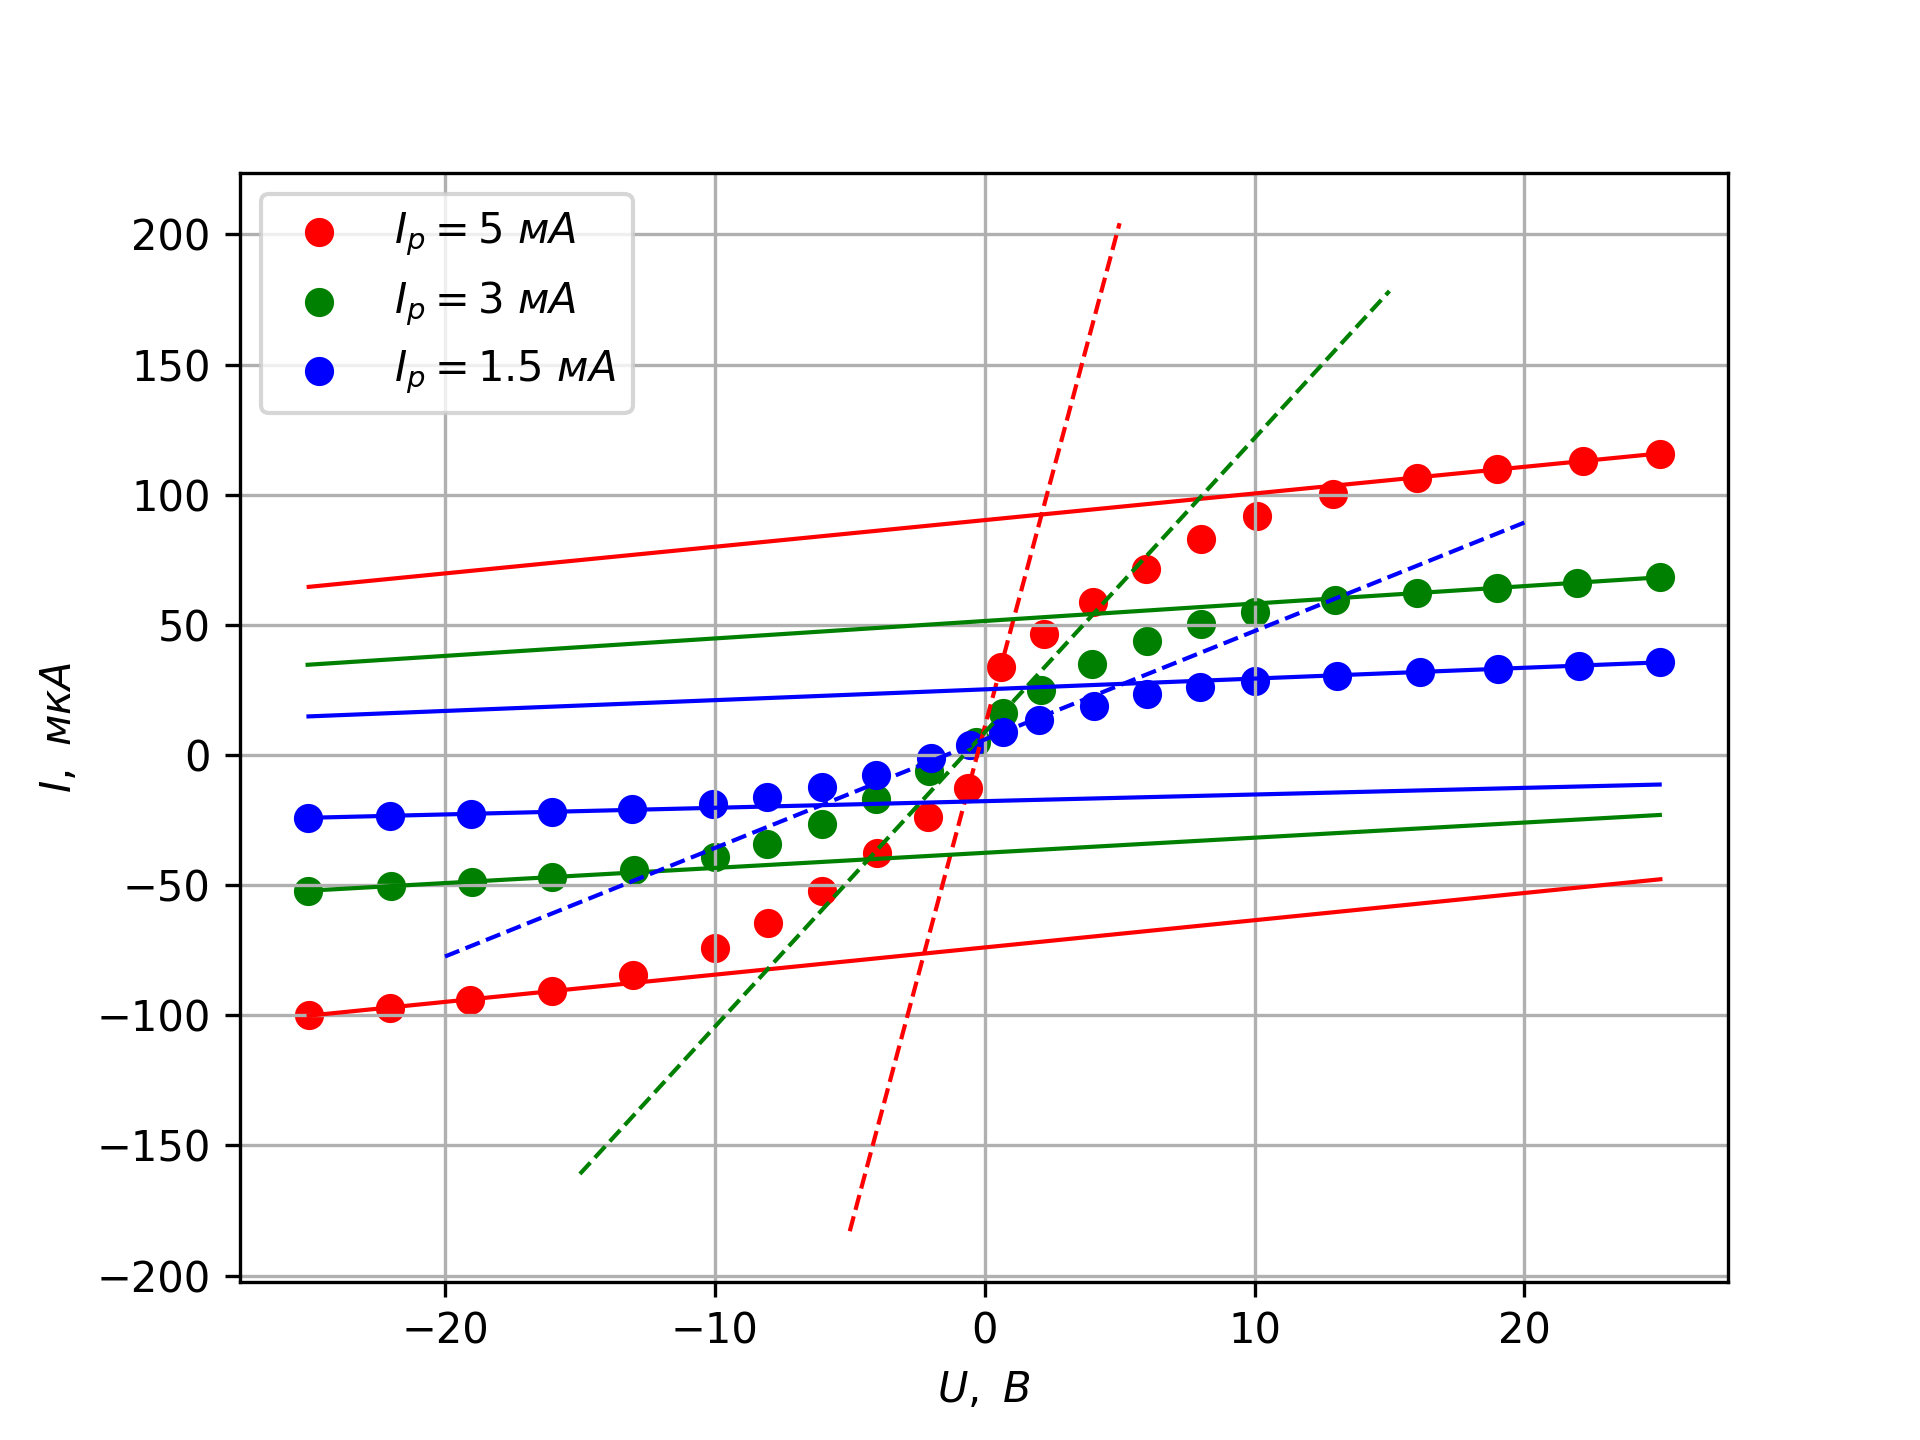
\includegraphics[scale=0.6]{images/351_2.png}
\caption{Вольт-амперная характеристика зонда для разных токов разряда $I(U)$}
\end{figure}

\begin{figure}[h]
\centering
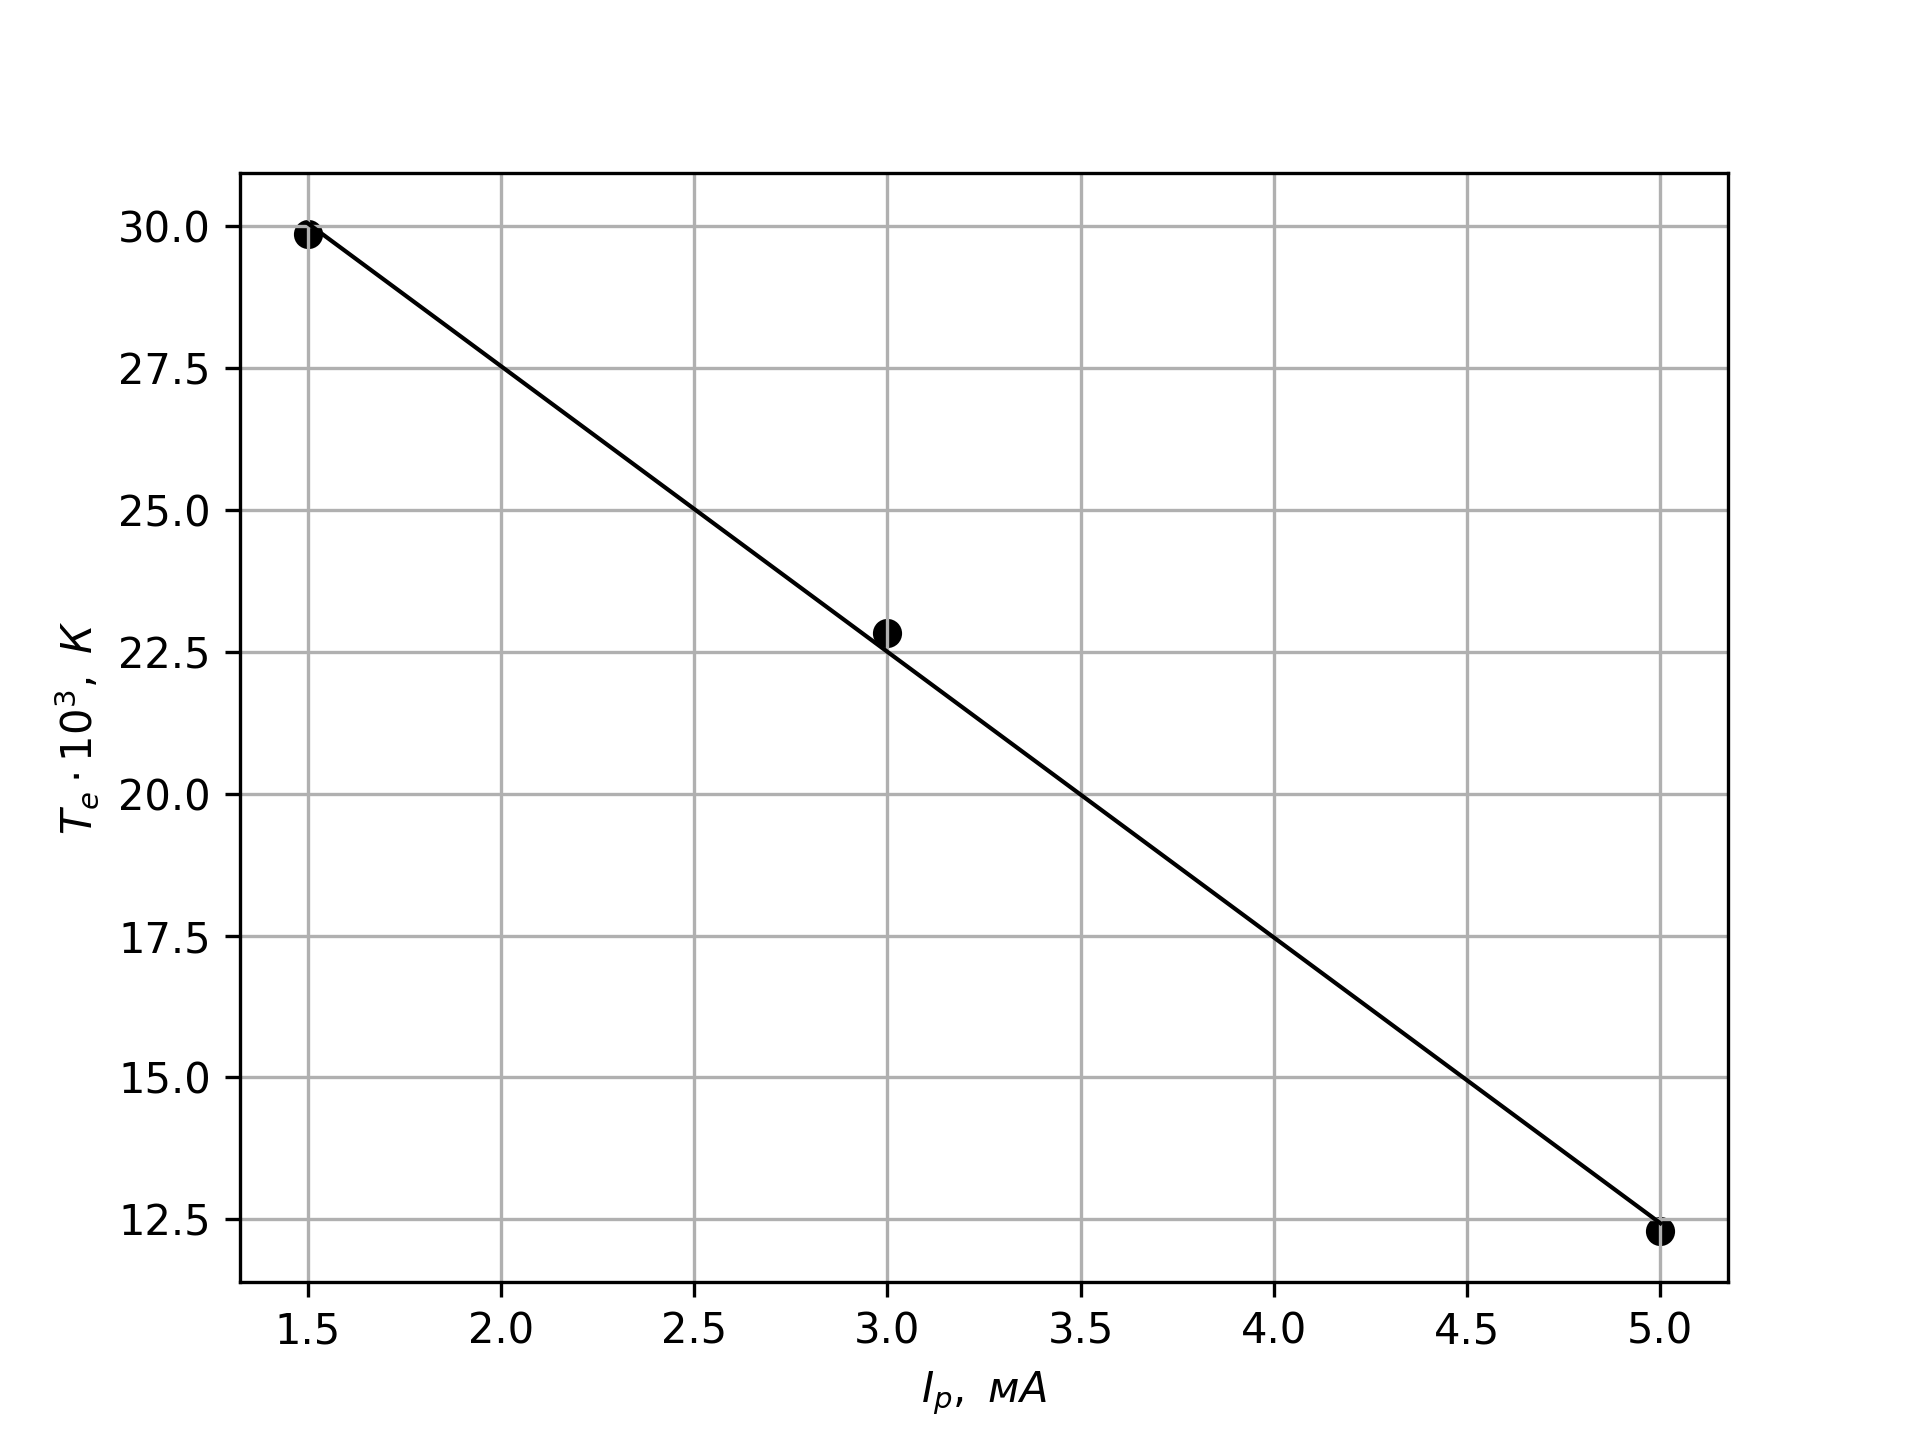
\includegraphics[scale=0.6]{images/351_3.png}
\caption{Зависимость $T_e(I_р)$}
\end{figure}

\begin{figure}[h]
\centering
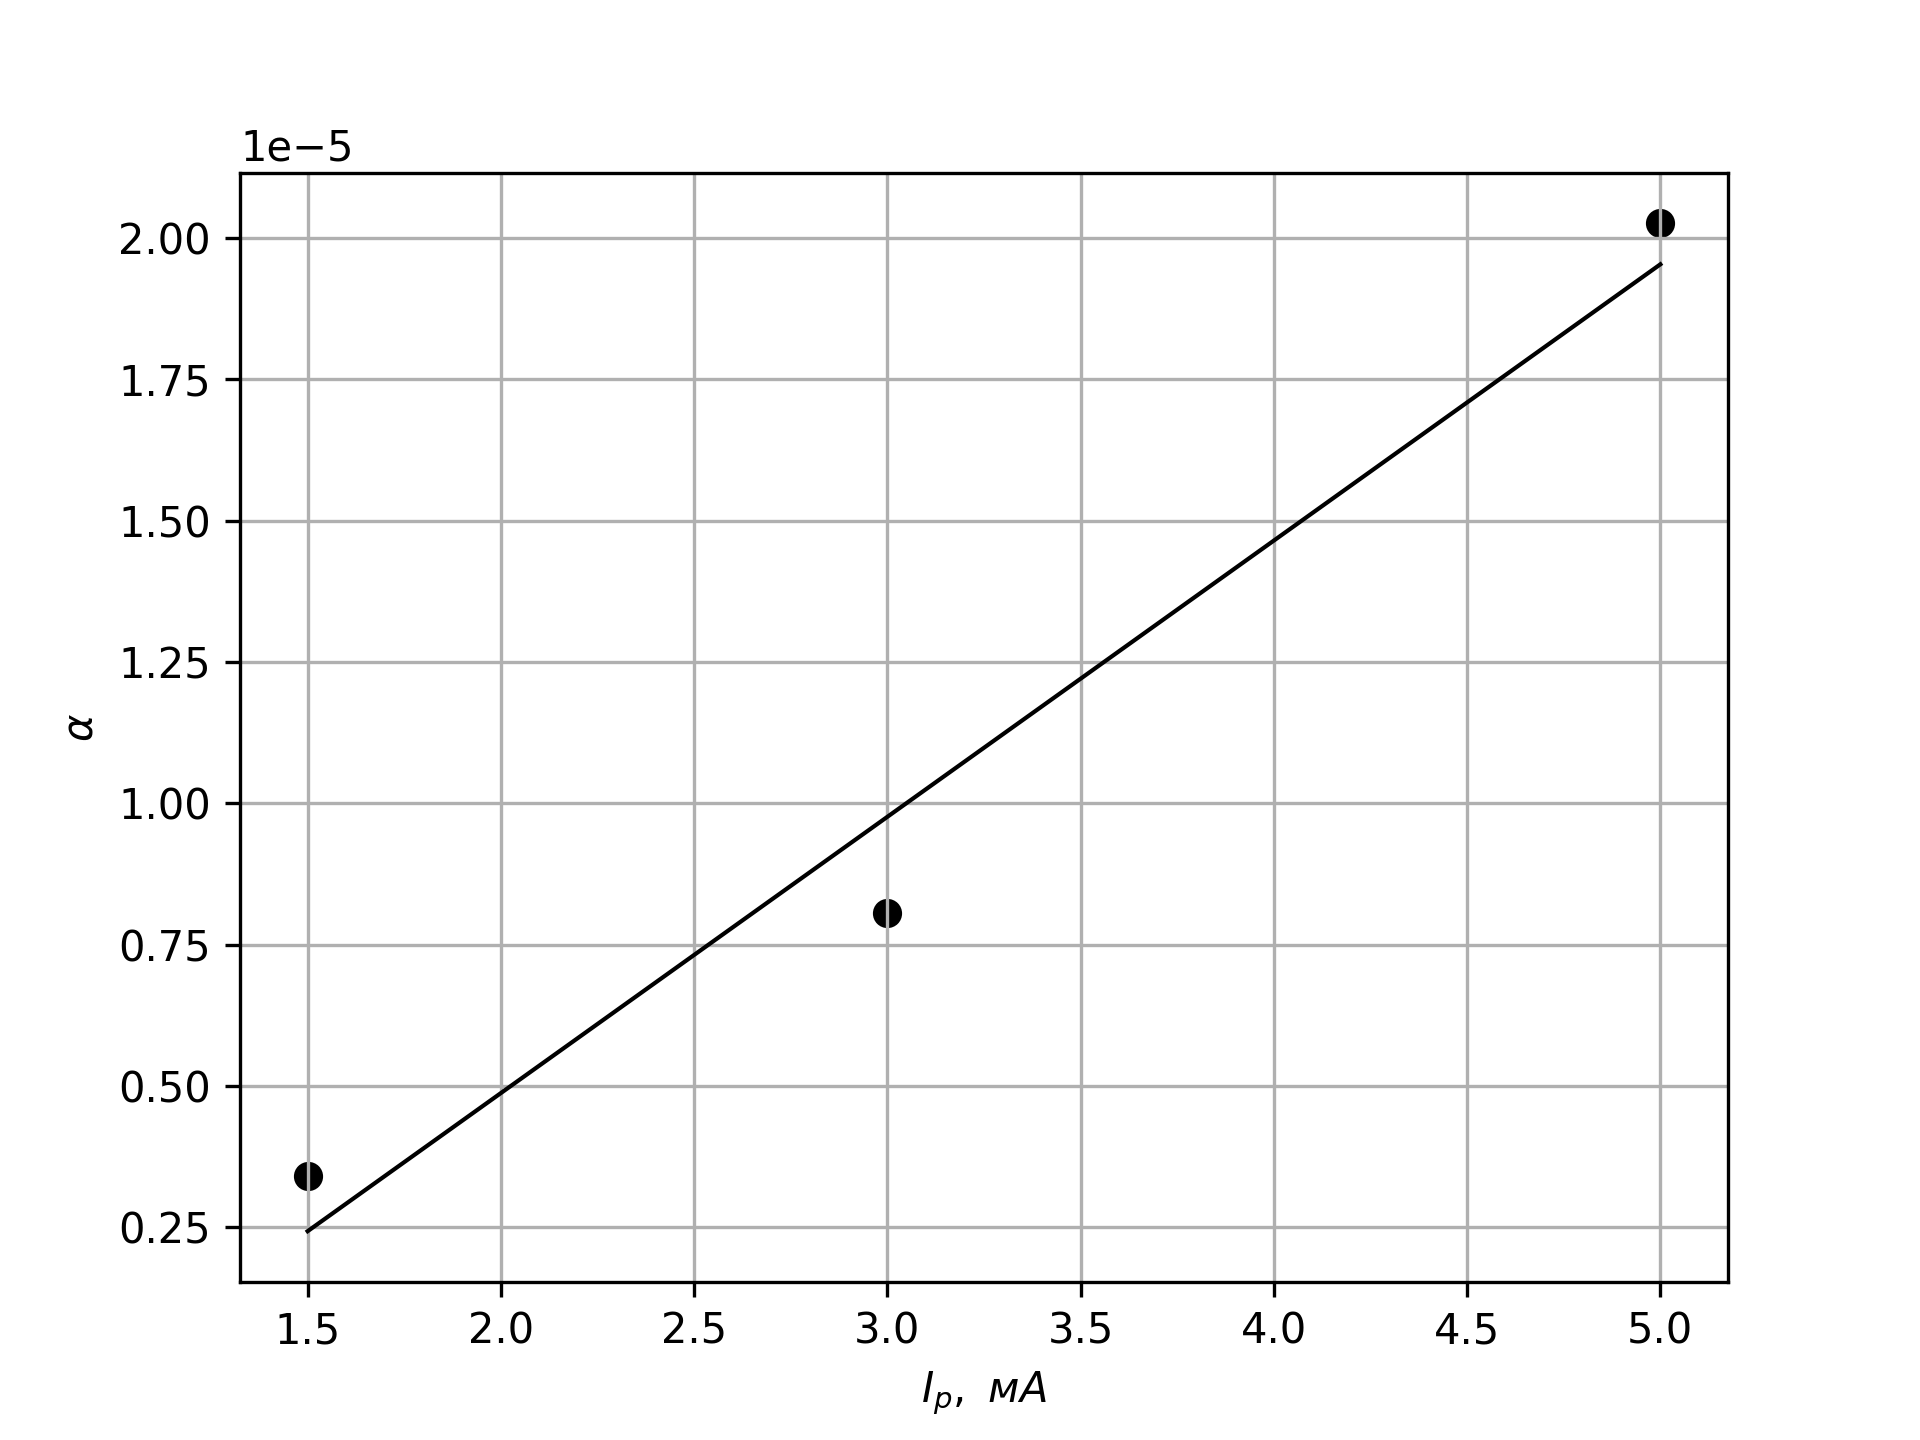
\includegraphics[scale=0.6]{images/351_4.png}
\caption{Зависимость $\alpha(I_р)$}
\end{figure}

\end{document}